\documentclass[10pt,a4paper,twocolumn]{article}
\usepackage{epsfig}

\setcounter{tocdepth}{2}

\begin{document}
\title{IgProf profiling tool}
\author{Giulio Eulisse, Lassi A. Tuura}
\maketitle

\begin{abstract}
  A fundamental part of software development is to detect and analyse
  weak spots of the programs to guide optimisation efforts.  {\em
  valgrind} and {\em oprofile} are two excellent tools that provide
  developers detailed information about their programs.  However they
  still leave holes to be filled.  {\em IgProf} is a new flexible
  debugging and profiling tool that can analyse large and complex
  applications.

  IgProf has three main components: a core profiler built on top of a
  generic event collector and dynamic function instrumentation tool, a
  number of profiling modules, and a utility to analyse the gathered
  data.  This article describes the profiler's features, output and
  implementation.
\end{abstract}

{\bf Keywords:} Profiling, performance profiler, memory usage, memory
leak, threads, shared library, C++, dynamic instrumentation, code
injection.

\tableofcontents

%%%%%%%%%%%%%%%%%%%%%%%%%%%%%%%%%%%%%%%%%%%%%%%%%%%%%%%%%%%%%%%%%%%%%%
%%%%%%%%%%%%%%%%%%%%%%%%%%%%%%%%%%%%%%%%%%%%%%%%%%%%%%%%%%%%%%%%%%%%%%
%%%%%%%%%%%%%%%%%%%%%%%%%%%%%%%%%%%%%%%%%%%%%%%%%%%%%%%%%%%%%%%%%%%%%%
\section{Introduction}

Three typical programming problems, immediately after being unable to
compile or run the program in the first place, are: {\em it's too
slow}, and {\em it uses too much memory}, and {\em it's both too slow
{\bf and} uses more memory than any realistic machine has.}  The
obvious solutions of buying a faster computer, more memory, or a
faster computer with more memory often yield only limited and passing
relief: the capacity of programmers to consume resources frequently
exceeds not only the supply but also the growth of the supply of those
resources.  The present shortage of well-established enemy nations and
lavish government grants has caused additional funding shortfalls.

The developer is therefore faced with a major ordeal: debugging and
optimising the code.

%%%%%%%%%%%%%%%%%%%%%%%%%%%%%%%%%%%%%%%%%%%%%%%%%%%%%%%%%%%%%%%%%%%%%%
\subsection{Profiling}

Optimization and debugging are tedious work to be done; some even
report it to be impossible.\footnote{Bruce Leverett is reported to
have written in ``Register Allocation in Optimizing Compilers'': But
in our enthusiasm, we could not resist a radical overhaul of the
system, in which all of its major weaknesses have been exposed,
analyzed, and replaced with new weaknesses.}  To ease this painful
task a number of tools have been developed and new ones are being
continuously written.  To name just a few, {\em gdb}, {\em valgrind}
and {\em oprofile}, cover a large spectrum of what is generally needed
to debug and profile our code.

It is crucial to have excellent profiling tools in order for a
developer to be able to focus on real, not imagined problems.  It is
not worth optimising a piece of code which only takes 1\% of the
execution time or memory if some other part consumes 35\% of them.
It is important that the tools point developers quickly and
effectively to the real source of the problems.

Profiling a program gives a quantified answer to the question ``How
much does each function in this program consume resource X?''  The
resource may be for example run-time (performance profile), amount of
memory allocated (memory profile), thread locking primitives (lock
contention profile), or system resources such as file descriptors.  If
the program should free the resources is has acquired, such as memory,
profiling can also tell where resources are leaked.

A common approach to performance profiling is event sampling: the
program execution location is sampled every once in a while, either
through instrumenting the code (e.g. at compile time), or by
statistical sampling (e.g. \verb|SIGPROF| signal or non-maskable
hardware interrupt).  The position within the program is recorded and
stored in a data structure which may be either hierarchical or flat.
Over a long run period the distribution of these samples produces a
fairly reliable indication where most of the time was spent.

Resource profiling is in fact analogous to performance profiling.  The
events to be sampled are calls from the program to acquire and release
resources, for instance to \verb|malloc()| and \verb|free()| memory
management functions.  The only difference is the profiler counts
memory allocated and freed, not just the number of ``ticks.''

%%%%%%%%%%%%%%%%%%%%%%%%%%%%%%%%%%%%%%%%%%%%%%%%%%%%%%%%%%%%%%%%%%%%%%
\subsection{Existing Open-Source Tools}

Before describing igprof we shall briefly cover a number of existing
open-source tools.  They have been an inspiration in developing our
own tool; we have sought to complement, not duplicate their
functionality.  In fact igprof started as an attempt to improve some
of the existing tools.

\subsubsection{valgrind}

Valgrind~\cite{valgrind} is a memory debugger for Linux systems.  It
only supports IA32 (i386-family) architecture.  At program start-up it
captures the execution and runs the program on a virtual IA32
processor.  It can be used with almost any ELF-based executable.  By
simulating the whole CPU, valgrind is able to track every memory
operation and track every bit written to and read.  This information
is used to generate warnings when uninitialised values are used,
accesses outside valid memory and leaks.  These days the tool has been
extended to support an impressive range of ``skins'' from cache
performance analysis to discovering synchronisation race conditions.

\subsubsection{oprofile}

Oprofile~\cite{oprofile} is a kernel level profiling facility.  It
uses debugging even registers that exist on most modern CPUs; when a
predetermined limit of events is exceeded, the CPU generates a
non-maskable interrupt.  Oprofile kernel module records which program
and where in that program the even occurred.  By sampling the system
and the programs for a while a fairly accurate profile is generated.
The choice of events that can be monitored is very rich on modern
CPUs and includes a variety of hardware-level details.

\subsubsection{jprof}

jprof~\cite{jprof} is a small performance profiler developed by the
Mozilla~\cite{mozilla} project to allow the browser to be profiled by
itself.  It uses standard \verb|SIGPROF| signals for sampling and can
be injected into programs with the \verb|LD_PRELOAD| mechanism, thus
requiring no instrumentation.

%%%%%%%%%%%%%%%%%%%%%%%%%%%%%%%%%%%%%%%%%%%%%%%%%%%%%%%%%%%%%%%%%%%%%%
%%%%%%%%%%%%%%%%%%%%%%%%%%%%%%%%%%%%%%%%%%%%%%%%%%%%%%%%%%%%%%%%%%%%%%
%%%%%%%%%%%%%%%%%%%%%%%%%%%%%%%%%%%%%%%%%%%%%%%%%%%%%%%%%%%%%%%%%%%%%%
\section{Using IgProf}

IgProf is designed to produce results much like gprof~\cite{gprof}.
Technically the implementation is very different, but results ``feel''
similar.  This means igprof produces a hierarchical profiling result,
so you can see both how much each individual function contributes and
how much entire call trees contribute.  When functions are called from
many different contexts you can see the contribution of each call
context separately.

\subsection{Getting IgProf}

IgProf is available as a CMS~\cite{cms} SCRAM~\cite{scram} project at
CERN.  It is released as free software under the GPL license; as it
requires no program instrumentation, anyone can use it.  You can also
download the software directly from CVS and build it yourself if you
would rather not use SCRAM.  However as the latter is quite easy,
there is really no reason not to use SCRAM.

If you are already a CMS software developer, you do not need to do
anything to get igprof: it is automatically part of the configuration
of nearly all CMS software projects.

Otherwise if you are at CERN, or have CMS software installed locally,
you can get IgProf into your environment with:

{\small\begin{verbatim}
  cd /afs/cern.ch/cms/Releases
  cd IGNOMINY/IGNOMINY_1_9_0/src
  eval `scram runtime -sh`    # bourne shell
  eval `scram runtime -csh`   # c-shell
\end{verbatim}}

If you cannot do either of the above, you can
\begin{itemize}
  \item Install SCRAM~\cite{scraminstall}
  \item Download IGNOMINY project~\cite{projectdownload}
  \item Setup the project area: \verb|scram setup|
  \item Build the project: \verb|scram build|
  \item \verb|eval `scram runtime -sh`|
\end{itemize}

\subsection{Getting Started Quickly}

It is not necessary to instrument the program for profiling in any
way.  Any program can be profiled as long as they are not statically
linked.  It is not necessary to compile with debugging information.
The profiler automatically detects if the program is multi-threaded,
and if so, automatically enables profiling of all threads as they are
created.  Code for all shared libraries is automatically profiled,
including dynamically loaded ones.

To test the profiler, you can try something like this:
{\small\begin{verbatim}
  igprof --debug --full ls
\end{verbatim}}

This will profile the \verb|ls| program using all currently available
profiling modules, including leak detection.  The \verb|--debug|
option produces more verbose output from the profiler itself; the most
useful part of that output is the name of the output file it produces
at the end of the run (\texttt{igprof.\textit{processid}}).  Use the
\verb|--help| option to get a complete summary of available options.

For example, to performance profile ORCA \verb|writeDST| program:
{\small\begin{verbatim}
  cd Examples/ExProduction
  eval `scram runtime -sh`
  igprof -d -pp writeDST -c orcarc.writeDST
\end{verbatim}}

At the end of the run the program will print out:
{\small\begin{verbatim}
  *** IgProf: exit() called, dumping state
  *** IgProf: dumping state to igprof.32098
  *** IgProf: igprof quitting
\end{verbatim}}

\subsection{Possible Measurements}

IgProf can currently profile performance (\verb|-pp| option), memory
usage (\verb|-mp|) and file descriptor usage (\verb|-fd|).  The memory
profiler can track the total amount of memory allocated, the largest
block of memory allocated, the amount of live memory left at exit, and
the maximum live memory at any point.  In leak check mode (\verb|-cl|)
all live blocks at the end are reported, with the live memory at the
end counts indicating how much each function leaked memory.  The file
descriptor profiler can track the number of file descriptors used,
live descriptors at exit (leaks), and maximum number of live
descriptors at any point.

Any number of these profiles can be enabled simultaneously---it is
perfectly viable to enable all of them at once.  This is particularly
useful if the program is very large and takes a long time to run, for
instance several hours or days.  Enabling more than one profiler
module of course introduces some skew as each profiler consume
resources themselves.  The core profiler disables all accounting while
within any profiler modules, so the effect is minimal, but it still
happens that the performance profiler generates hits on other modules.

\begin{figure*}[!htbp]
{\small
\begin{verbatim}
     53553180   50642044   5/5     PersistentJetFinder::reconstruct() (.../ORCA_8_0_1_pre1/lib/...)
 [0] 50642044   50226044   5     JetFinderEcalPlusHcalTowerInput::prepareInput(RecEvent const*) (...)
      5863168          0   5/62    BaseRecItr::BaseRecItr[not-in-charge](RecoQuery const&) (writeDST) [952]
    229962815          0   5/49    LazyObserver<RecEvent const*, int>::check() const (writeDST) [732]
        36864          0   5/14    std::vector<VJetableObject*, std::... >::_M_insert_aux(...
            0          0   5/5     JetableObject<EcalPlusHcalTower>::JetableObject[in-charge](...) (...)
     62299760     416000   5/547   RecQuery::operator RecConfig const&() const (.../COBRA_7_7_1_...)
\end{verbatim}}
\caption{Sample igprof results for one function}
\end{figure*}

\begin{figure}[!htbp]
\begin{center}
  \mbox{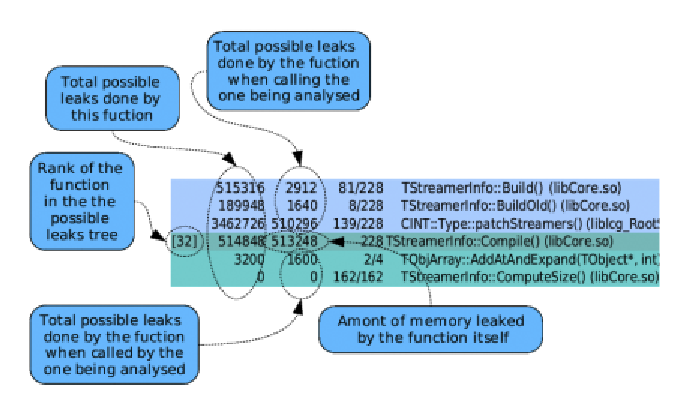
\epsfig{file=igprof-output.eps,width=.50\textwidth,clip=}}
  \caption{Reading profiling results}\label{fig:result}
\end{center}
\end{figure}

\subsection{Analysing the Results}

The file produced by igprof is a raw trace file that you analyse with
\verb|igprof-analyse| program to produce the final profiling result.
You can run \verb|igprof-analyse| several times for different ``cuts''
of the profiling results; you don't need to re-run the profiled
application for this.  The analyser can produce the output as a plain
text table, HTML, or XML.  Opening the HTML version in a web browser
is the most convenient way to navigate the call trees.

\subsection{Interpreting the Results}

igprof output resembles that of gprof so its output conventions
documentation may be helpful to read first~\cite{gprofresult}.

The following explanation assumes memory leak checking.  If you are
measuring something else, adjust the explanation correspondingly for
CPU time or memory allocated. The output format is the same, just the
meaning of the numbers is different.

The result file is made of sections like shown in Figure~\ref{fig:result}.

Each section describes the statistics for one function, the primary
function, surrounded by secondary functions.  Above the primary
function are the callers: the functions that called the primary
function.  Below the primary function are the callees: the functions
the primary function called. The line that begins with a bracketed
number, here '[0]', indicates the primary function; the number in the
brackets indicates the function's index in the statistics.  The
smaller the index is, the higher the function was in cpu time usage,
memory usage or leakage.  The next columns are the statistics
explained in more detail below. The first text column tells the name
of the function, here
JetFinderEcalPlusHcalTowerInput::prepareInput(RecEvent const*),
followed by the name of the module where it was found, here
writeDST.  The callers and callees give the index of the function after
the module name, such as the '[952]' and '[732]' in the first two
callees here, to help in navigating in the output.

For the primary function line the first statistic is the sum of the
memory leaked by the function and all its callees, here 50642044.  The
second statistic is the amount of memory leaked directly by the
function itself, here 50226044.  So in this case we can already see
that most of the memory was leaked by the function itself. The third
statistic is the number of unique call paths that resulted in a leak,
here 5. Note that this is not the number of calls that resulted in a
leak, but the number of unique call paths: there were five different
calls stacks with this function in the stack. There could have been
thousands of such calls. (FIXME: allocations or leaks, can't be leaks
if child entries are zero?)

For the secondary functions the statistics are slightly different. The
first statistic is the total amount of memory the function leaked in
any call path. The second statistic is the amount leaked when the
primary function was also in the call stack. For callers this is the
amount of memory the caller leaked through the primary function. For
callees it is the amount the primary function leaked through that
callee. So the second number is always less than the first one. The
third number pair is first the number of calls paths including the
primary function, and then total number of calls to the function.

In our example output, PersistentJetFinder::reconstruct() leaked a
total of 53553180 bytes, of which most, i.e. 50642044 bytes, was due
to our example main function. All the memory leaked by the children of
our example main function went through RecQuery::operator RecConfig
const\&() const, a total of 416000 bytes (= 50642044 -
50226044). However, that function leaked a total of 62299760 in 547
different call paths; five of those call paths were due to this
primary function.

For another example below, TStreamerInfo::Compile() leaked 514848
bytes, of which 513248 directly. This was from 228 different call
paths. Of those, 2912 bytes were result of 81 call paths from
TStreamerInfo::Build() (of 228 call paths resulting in 515316 bytes of
leaks in the latter). 1640 bytes were leaked for calls from
TStreamInfo::BuildOld() in 8 call paths. 510296 bytes, the majority,
was from calls to CINT::Type::patchStreamers(). Majority of the memory
was leaked directly. However TObjArray::AddAtAndExpand() leaked 1600
bytes in two call paths (out of four call paths and 3200 bytes leaked
in total to that function). Memory was allocated but not leaked via
'TStreamerInfo::ComputeSize()'; there were 162 call paths to the
latter but they all came from this function.

%%%%%%%%%%%%%%%%%%%%%%%%%%%%%%%%%%%%%%%%%%%%%%%%%%%%%%%%%%%%%%%%%%%%%%
%%%%%%%%%%%%%%%%%%%%%%%%%%%%%%%%%%%%%%%%%%%%%%%%%%%%%%%%%%%%%%%%%%%%%%
%%%%%%%%%%%%%%%%%%%%%%%%%%%%%%%%%%%%%%%%%%%%%%%%%%%%%%%%%%%%%%%%%%%%%%
\section{IgProf Implementation}
\subsection{Overview}

IgProf has three main components: a core profiler built on top of a
generic event collector and dynamic function instrumentation tool, a
number of profiling modules, and a utility to analyse the gathered
data.

Requirements (from below)

General structure

Output + separate analysis


\subsection{Profiler Core}

Profiler, hook library, counter traces, initialisation, locking,
thread handling, exit capture.

\subsection{Injecting the Profiler}

Preload, possibly injection, automatic activation

\subsection{Trapping Calls and Signals}

Describe the call trap mechanism, signal handlers, thread capture and
handling for performance profiling.  Calling to the original function.

\subsection{Maintaining Counters and Resources}

Describe the hook trace trees, memory allocation via mmap().

\subsection{Adding Profiler Modules}

Describe how to define new profiler modules.

%%%%%%%%%%%%%%%%%%%%%%%%%%%%%%%%%%%%%%%%%%%%%%%%%%%%%%%%%%%%%%%%%%%%%%
%%%%%%%%%%%%%%%%%%%%%%%%%%%%%%%%%%%%%%%%%%%%%%%%%%%%%%%%%%%%%%%%%%%%%%
%%%%%%%%%%%%%%%%%%%%%%%%%%%%%%%%%%%%%%%%%%%%%%%%%%%%%%%%%%%%%%%%%%%%%%
\section{Advanced Use}

Options, tracing by self/accumulated, correlating results from
multiple options, diffing results (persistent leaks).  Using
performance profiler to find graphics problems.  Using real-time
profiling instead of process-time profile.

\subsection{Tracing Problems}

Finding problem cause when one function allocates, another frees.
When an object is allocated, and a member is rotated, the leak is
blamed on the object, but the real error is where the member is
rotated (last copy not freed in destructor/loop exit).  Common
misleading issues, std pool allocators.  When functions don't seem to
get hit by statistical hits.

\subsection{Common Mistakes}

Vectors of pointers to object, forgetting to delete the object.
Forgetting to delete an object in a destructor.

%%%%%%%%%%%%%%%%%%%%%%%%%%%%%%%%%%%%%%%%%%%%%%%%%%%%%%%%%%%%%%%%%%%%%%
%%%%%%%%%%%%%%%%%%%%%%%%%%%%%%%%%%%%%%%%%%%%%%%%%%%%%%%%%%%%%%%%%%%%%%
%%%%%%%%%%%%%%%%%%%%%%%%%%%%%%%%%%%%%%%%%%%%%%%%%%%%%%%%%%%%%%%%%%%%%%
\section{References}
\begin{thebibliography}{9}
  injlib Jerry Richter WSJ 1994

  injectso http://www.securereality.com.au/

  paradyn dyninst http://www.dyninst.org/

  mach\_inject / mach\_override
  http://rentzsch.com/mach\_inject/
  http://rentzsch.com/mach\_override/
  http://cvs.sourceforge.net/viewcvs.py/extendamac/code/mach\_inject/mach\_inject.c?rev=1.1.1.1\&view=auto

\end{thebibliography}
\end{document}




%%%%%%%%%%%%%%%%%%%%%%%%%%%%%%%%%%%%%%%%%%%%%%%%%%%%%%%%%%%%%%%%%%%%%%
%%%%%%%%%%%%%%%%%%%%%%%%%%%%%%%%%%%%%%%%%%%%%%%%%%%%%%%%%%%%%%%%%%%%%%
%%%%%%%%%%%%%%%%%%%%%%%%%%%%%%%%%%%%%%%%%%%%%%%%%%%%%%%%%%%%%%%%%%%%%%
%%%%%%%%%%%%%%%%%%%%%%%%%%%%%%%%%%%%%%%%%%%%%%%%%%%%%%%%%%%%%%%%%%%%%%
%%%%%%%%%%%%%%%%%%%%%%%%%%%%%%%%%%%%%%%%%%%%%%%%%%%%%%%%%%%%%%%%%%%%%%
%%%%%%%%%%%%%%%%%%%%%%%%%%%%%%%%%%%%%%%%%%%%%%%%%%%%%%%%%%%%%%%%%%%%%%
\section {Introduction}

We all know that the typology of problems one encounters when
programming can be divided in three main areas:

\begin{itemize}
\item ``Ehi! My code runs slow!''
\item ``Ehi! My code requires 1 GB of RAM!''
\item ``Ehi! My code is slow {\em AND} requires 2GB of memory!''
\end{itemize}

The typical solutions to this kind of problem fall in three main area,
especially when we are talking about international institutions:

\begin{itemize}
\item ``Buy a faster computer''
\item ``Buy more memory''
\item ``Buy a faster computer with even more memory''
\end{itemize}

However the recent recession and the end of Cold War made this
approach rather difficult to follow.  The lack of well established
communist countries with nuclear war-heads made the search for
fundings more complicate especially for those institutions with
``Nuclear'' in their name.  Although someone tried to replace USSR
with GRID it seems that a ``third way'' in computer programming has to
be explored.

We actually have to start debugging and optimizing our code.

\section{Profiling}

Optimization and debugging is a tedious work to be done, if not
impossible according to some [\cite{JokesAboutProgramming}] theories,
however, to ease this job a number of tools where written and are
still being developed. {\em gdb}, {\em valgrind}, {\em oprofile} just
to name a few, cover a large spectrum of what is generally needed to
debug and profile our own code.

It is actually important to have a good tools for profiling because
often this way we can focus our attention of the real problem and not
be distracted by less important parts: there is no interest in
performing optimization on something which takes only 1\% of the time
or of the memory when somewhere else we are using 99\% of the
resources..
 
Usually when profiling a program we are interested in three different
things:

\begin{itemize}
\item Understanding in which function we spend the most amount of time,
  and if this is avoidable (performance profiling)
\item Understanding in which function we allocate more memory (memory
  profiling)
\item See if there is any allocated memory left behind by mistake
  (leaks hunting)
\end{itemize}

The common approach for performance profiling is the so called event
sampling.  The program execution is is interrupted every once in a
while in a number of different ways (code instrumentation,
\verb|SIGPROF| signal, non-maskable hardware interrupt) and the
position within the program is stored in some data structure, that can
be either flat, or hierachical. In the long run, the distribution of
this information about the forced stops of a the program, produce the
distribution of where most of the time was spent. The problem of
memory profiling is actually analogous to that of performance
profiling.  Actually, it is a superset of it and the structure used to
keep track of it can actually be used, almost untouched to keep the
information used by the performance profiler. The external event used
in performance profiling to obtain the distribution of computing time
among different functions in the case of memory profiling is the act
of intercepting allocation and free operations. The only difference
between the two is that in this case we insert in the data structure
the amount of memory allocated/freed, rather than increment a counter.

\section{Open Source profiling tools} 

Before starting to talk about igprof, we would like to briefly describe some
great opensource tools that have been of inspiration for developing our own
profiling tool which was actually started in the attempt of completing and
integrating the present opensource possibilities.

\subsection{valgrind}

Valgrind is an open source memory debugger for linux running on IA32
architecture. It provides a virtual machine able to run IA32 code
which can be used to run almost any {\em ELF-based} executable.  By
simulating the whole CPU, {\em valgrind} is able to track every single
memory operation and to keep track on every single byte read or
written to memory.  These information can be therefore used to keep a
complete log of leaks, uninitialized memory reads/write and also cache
performance (by the simulation of the behavior of L1 caches and
unified L2 cache).

\subsection{oprofile}

Oprofile is a kernel level profiling facilities, it uses non maskable
interrupts generated by the CPU to obtain, via sampling, the
information about processing power distribution and many other
hardware related information.

\subsection{jprof}

jprof is a small performance profiler developed by the ``mozilla''
project for self profiling purposes. It uses signal()s in place of
hardware interrupts to do the sampling and the \verb|LD_PRELOAD|
mechanism to be attached unintrusively to the program to be profiled.

\subsection{Requirements for a profiling tool}

As a memory debugger, valgrind does an excellent job in finding memory
leaks and general memory errors, however, it is too slow to be of
practical use when profiling computational intensive applications and
it does not provide (yet, I might add, as I know this is planned)
quantitative informations about memory usage and
allocations. Moreover, it is only available on x86 system and it is
limited to the instruction set present in the emulation. Oprofile, on
the other end doesn't have (yet) a tree view of the profiling
informations and most important of all is intrusive at kernel level
This is drawback expecially in production farms, where the
administrator are usually not very happy about having kernel level
extensions. Jprof could be seen as a solution to this problem, as it
is completely unintrusive, but it lacks (since they are out of its
scope) of all the memory profiling features we might want to have. So
here it is our list for the ``most wanted'' features of our ``ultimate
profiling utility''

\begin{itemize}
\item ``It must be fast enough to profile our (CMS experiment) software''
\item ``It must be completely unintrusive (ala valgrind) and easy to use''
\item ``It must be able to profile performances''
\item ``It must be able to profile memory usage''
\item ``It must give us a fast way to detect leaks''
\item ``It must give us call tree information''
\end{itemize}

Luckily enough most of the low level features we need to get such
debugging/profiling information are already present in {\em glibc}, so
the profiler itself, at least as a first order approximation, is just
a matter of getting all of them together, with an optimized structure
to keep the information collected at runtime and a nice layout for the
output. This is the the history about how {\em igprof} (the ignominous
profiler) was born.

\subsection{General structure of the profiler}

We define a profiler as a phantom object, which is loaded alongside
the program to be profiled which observes profiling ``events''. A
profiling event is made up of the stack trace of where it happened and
carries with it some information about the event itself. An event can
be istantaneous, or could last in time. In the latter case it is
actually made of two events: one that notifies the start, the other
that notifies the end. After the profiler is attached to a program it
begins to wait for events. According to the different options it has
been invoked with these events can be memory
allocations/deallocations, timer interrupts, instrumented code calls
or more \footnote{at the time this article has been written, only the
first two kinds of events are actually fully implemented.}. When one
of these events occur the program execution stops and the information
about the backtrace is retrieved, filtered according to the event kind
and to optional extenal configuration and inserted in the profiling
data structure. This data structure is, to a first order, a tree in
which each node represents one entry of the stack trace. This is done
in order to avoid keeping track of every single event that happend in
the execution of a program but rather all the information is merged so
that events happened within the same execution path are actually
summed up. This is all we need for profiling instantaneous events like
the total number of bytes allocated or the hits of a fixed interval
timer. If we want to keep track of leaks or of the maximal heap size
for we need one more data structure in order to keep track of ``live
allocations''. This is because allocations are non-instantaneous
events that last in time and have notify their start and their end
\footnote{an ``allocation event'' starts when the memory is allocated
via malloc and ends when the memory is freed by free ()}. In such a
list of live events one has to keep track not only of an id
\footnote{the pointer to the allocated memory, for example} that
allows to ``close'' an event, but also of the end node in the tree
structure which refers to that entry. In this way when an event is
close we are able to modify the tree structure so that it behaves
accordingly. For example, in the case of leak hunting, once a memory
allocation event is closed, we need to subtract its contribution to
the tree.

\subsection {Convenient output format}

Until now, we have talked about in memory structure for the profiling
data, which is basically a tree. Even though we could dump to disk the
raw tree structure itself (for example using XML) this is not very
handy, has the tree could be very deep or unbalanced and more
important one function could be called in different callpaths, while
we could be interested in the sum of all the results of all these
branches. So, it is more convenient to use a gprof like structure for
the output, in which the output is made of many blocks, one for each
different function in the tree. This means that each one of these
blocks gives information about one function, its callees and its
children, no matter if these where in different callpath..

\section{Technical details}
\subsection{Injecting a library: the LD\_PRELOAD mechanism}

\textit{Posix} provides a very clean way of modifing and patching
executables in an unintrusive way. It is possible to preload (or
inject) one or more shared library in the execution space of a program
before the program itself starts to run by specifing it to the special
system environment variable \verb|LD_PRELOAD|.  Before a program is
executed, the runtime linker will load and map the libraries specified
in such a variable to the memory space of the program about to be run
and it will instanciate all the static objects defined within the
library. This allows to setup and initialize our profiling facility by
wrapping all the action required to do it in the constructor of a an
object being statically instanciated. This will allow to have it
working transparently with every program we want, written in any
compiled language with no code instrumentation at all. It also works
pretty much with all \textit{posix} compliant systems. Notice that
this approach is already used by valgrind or jprof.

\subsection{Intercepting malloc hooks: malloc callbacks}

Having detailed information about memory allocations was the original
reason for writing \textit{igprof}, as it is a feature which has not
been found on any of the profilers examined. In its current
implementation, igprof takes advantage of a special feature of glibc
(http://www.glibc.org), the Linux standard C library, which allows
hooking code into {\em malloc()}/{\em free()}/{\em memalign()}/{\em
realloc()}. It is enough to overwrite the correspondent symbols

\begin{itemize}
\item \verb|__malloc_hook|
\item \verb|__free_hook|
\item \verb|__memalign_hook|
\item \verb|__realloc_hook|
\end{itemize}

with custom code to be able track of every single memory
allocation/deallocation operation.

Besides keeping track of the amount of memory being allocated and
freed, we also obtain information about where this memory was
requested/disposed by looking at current stack trace, via
{\em backtrace()} function.

\subsection{Intercepting function calls, a generalization} 

glibc provides hooks for malloc() and free() because, being memory
related, those are the function one is usually interesed the
most. Sometimes though we might be interested in watching other
functions and for several reasons we might not be able to instrument
the code so that a ``profiling event'' is generated upon their call. A
possible, non intrusive, solution for this problem is to generate a
little wrapper library which has wrapper function with the same symbol
name of the function we want to trace. This wrapper function will be
responsible for generating the profiling event and then calling the
real code.  Once again, this is, possible thanks to \verb|LD_PRELOAD|
which will allow us to load this library before the real one so that
its symbols will be resolved before the real one. The wrapper code can
then use dlsym with the \verb|RTLD_NEXT| option to get the real code.

%%% The information fetched in this way is then stored in a tree structure
%%% in which every node is an entry in the of the stack trace and contains
%%% the total amount of memory being allocated from that function and all
%%% the functions it calls.  This information is already enough to keep
%%% track of the total amount of allocations performed by a program. This,
%%% however, even if it's a good start, is still a quite unusable
%%% information, as ``for'' loop which allocates and delete 1 byte of
%%% memory 100 hundred times would still appear with a weight of 100 in
%%% the tree.

%%%\begin{verbatim}
%%%...
%%%for (int i = 0; i < 100; i++)
%%%{
%%%delete new char;
%%%}
%%%...
%%%\end{verbatim}

%%% A more interesting quantity to analize is the maximum heap size per
%%% function, which is the maximum amount of memory that was allocated by
%%% a fuction at once during the whole program execution.  For example,
%%% the function a() of , would have a weight of 1, rather than a In order
%%% to be able to track the disposal of such allocations, moreover, we
%%% keep a map of all the live allocations and the leaf node in which they
%%% where stored in the

\subsection{memory leaks checker}

The leak checker which comes with igprof was written to address a
particular issue in the \textit{ORCA} particle tracks reconstruction
software, which was occupying to much memory, so we decided to add
igprof the ability to hunt for non freed memory. The memory leaks
check tool can be activated on the side of the memory profiler. It
keeps a flat table of all the live allocations found in the
system. If, when a process exits there are entries in the table they
are pointed out as possible leaks. This is not always the case,
because some this memory could be allocated and never freed, but
actually used for the whole program, letting the exit code perform the
deallocation. However this information is still useful to do leak
hunting and most important results can be obtained in a reasonable
amount of time, which is not the case for more accurate memory
debuggers like valgrind. A way to eliminate false friends is to check
the time dependency of such leaks. If a possible leak has the tendency
to increase as times goes on, it is very likely to be an actual
leak. If it does not then it's either not a leak, or it will be most
likely swapped out by the memory management system when the system
goes low on available memory.

\end{document}
